\documentclass{article}
\usepackage[12pt]{extsizes}
\usepackage[utf8]{inputenc}
\usepackage{amsmath}
\usepackage{amsfonts}
\usepackage{amssymb}
\usepackage{tabularx}
\usepackage{multirow}
\newcommand{\RomanNumeralCaps}[1]
{\MakeUppercase{\romannumeral #1}}
\usepackage{cmap} % для кодировки шрифтов в pdf
\usepackage[T2A]{fontenc}
\usepackage[russian]{babel}
\usepackage{graphicx} % для вставки картинок
\usepackage{amssymb,amsfonts,amsmath,amsthm} % математические дополнения от АМС
\usepackage{indentfirst} % отделять первую строку раздела абзацным отступом тоже
\usepackage[outdir=./]{epstopdf}
\usepackage{listings}
\usepackage{color} %red, green, blue, yellow, cyan, magenta, black, white
\definecolor{mygreen}{RGB}{28,172,0} % color values Red, Green, Blue
\definecolor{mylilas}{RGB}{170,55,241}
% Поля
\usepackage{geometry}
\geometry{left=2.5cm}
\geometry{right=1.5cm}
\geometry{top=1.5cm}
\geometry{bottom=2cm}

%%%%%%%%%%%%%%%%%%%%%%%%%%%%%%%    

\linespread{1.5} % полуторный интервал
\renewcommand{\rmdefault}{ftm} % Times New Roman
%\renewcommand{\rmdefault}{PT-Astra-Serif_Regular}
%\usefont{T2A}{PT-Astra-Serif_Regular}{m}{it}
\frenchspacing

% подключаем hyperref (для ссылок внутри  pdf)
\usepackage[unicode, pdftex]{hyperref}

% коррекция подрисуночной подписи
\usepackage{caption}
\captionsetup[figure]{labelsep=period} %Точка
%\captionsetup[figure]{labelsep=space}  %Пробел
%\captionsetup[figure]{labelsep=endash}  %Новый страндарт
\usepackage[figurename=Рисунок]{caption}
\usepackage{longtable}


\begin{document}
	
	\begin{titlepage}
		
		\begin{center}
			САНКТ-ПЕТЕРБУРГСКИЙ ГОСУДАРСТВЕННЫЙ ЭЛЕКТРОТЕХНИЧЕСКИЙ УНИВЕРСИТЕТ «ЛЭТИ» \\ИМ. В.И. УЛЬЯНОВА (ЛЕНИНА)\\
			\vspace{0.1cm}
			Кафедра Алгоритмической математики\\
			
			
			
		\end{center}
		
		\vspace{5cm}
		\begin{center}
			\begin{large}
				Лабораторная работа 3 \\
				"Численное дифференцирование"
			\end{large}
		\end{center}
		
		\vspace{5cm}
		
		\hspace{5cm} Студент гр.  0307 \hrulefill Латин Я.М.
		
		\vspace{0.5cm}
		\hspace{5cm} Преподаватель \hrulefill  Солнышкин С.Н.\\
		
		
		\vfill
		\begin{center}
			Санкт-Петербург\\
			2022
		\end{center}
		
		
	\end{titlepage}
	
	
	\newpage
	\tableofcontents
	\newpage
	\section{Задание}
	Сравнить точные значения $ f'(x_0), f''(x_0) $ с конечно-разностными первыми производными 1-го, 2-го и 4-го порядков точности и конечно-разностными вторыми производными 2-го и 4-го порядков точности, вычисляемыми по последовательно уменьшающимся вдвое значениям шага, если
	\( f(x)=\dfrac{2000}{(x^2-3x+92)},~x = 1 \)
	
	\section{Явные формулы и значения $ f'(x_0), f''(x_0) $}
	
	\begin{flushleft}
		\[f'(x) \dfrac{(2000(3-2x))}{(x^2-3x+92)^2},~f'(x_0) = 0.24691 \]\\
		
		\[f''(x)= \dfrac{4000\left(3x^2-9x-83\right)}{\left(x^2-3x+92\right)^3},~f''(x_0) = -0.48834\]
	\end{flushleft}
	
	\section{Первая конечно-разностная производная 1-го порядка точности}
		\begin{flushright}
			Таблица 1. Погрешности первой производной первого порядка точности.
		\end{flushright}
		
			\begin{table}[h!]
				\centering
				\begin{tabular}{|l|l|l|}
					\hline
					\multicolumn{1}{|c|}{$k$}  & \multicolumn{1}{c|}{$h_k$}       & \multicolumn{1}{c|}{$r_k$}    \\ \hline
					\multicolumn{1}{|c|}{17} & \multicolumn{1}{c|}{1.5259e-05} & \multicolumn{1}{c|}{3.7258e-06}  \\ \hline
					\multicolumn{1}{|c|}{18} & \multicolumn{1}{c|}{7.6294e-06} & \multicolumn{1}{c|}{1.8627e-06}  \\ \hline
					\multicolumn{1}{|c|}{19} & \multicolumn{1}{c|}{3.8147e-06} & \multicolumn{1}{c|}{9.3135e-07}  \\ \hline
					\multicolumn{1}{|c|}{20} & \multicolumn{1}{c|}{1.9073e-06} & \multicolumn{1}{c|}{4.6568e-07}  \\ \hline
					\multicolumn{1}{|c|}{21} & \multicolumn{1}{c|}{9.5367e-07} & \multicolumn{1}{c|}{2.3285e-07}  \\ \hline
					\multicolumn{1}{|c|}{22} & \multicolumn{1}{c|}{4.7684e-07} & \multicolumn{1}{c|}{1.1737e-07}  \\ \hline
					\multicolumn{1}{|c|}{23} & \multicolumn{1}{c|}{2.3842e-07} & \multicolumn{1}{c|}{5.7765e-08}  \\ \hline
					\multicolumn{1}{|c|}{24} & \multicolumn{1}{c|}{1.1921e-07} & \multicolumn{1}{c|}{2.7963e-08}  \\ \hline
					\multicolumn{1}{|c|}{25} & \multicolumn{1}{c|}{5.9605e-08} & \multicolumn{1}{c|}{-3.1642e-08} \\ \hline
					\multicolumn{1}{|c|}{26} & \multicolumn{1}{c|}{2.9802e-08} & \multicolumn{1}{c|}{2.7963e-08}  \\ \hline
					\multicolumn{1}{|c|}{27} & \multicolumn{1}{c|}{1.4901e-08} & \multicolumn{1}{c|}{-9.1247e-08} \\ \hline
					\multicolumn{1}{|c|}{28} & \multicolumn{1}{c|}{7.4506e-09} & \multicolumn{1}{c|}{-3.2967e-07} \\ \hline
					\multicolumn{1}{|c|}{29} & \multicolumn{1}{c|}{3.7253e-09} & \multicolumn{1}{c|}{-3.2967e-07} \\ \hline
					
				\end{tabular}
			\end{table}
		
			\begin{table}[h!]
				\centering
					\begin{tabular}{|l|l|l|}
						\hline
						
						\multicolumn{1}{|c|}{30} & \multicolumn{1}{c|}{1.8626e-09} & \multicolumn{1}{c|}{-3.2967e-07} \\ \hline
						\multicolumn{1}{|c|}{31} & \multicolumn{1}{c|}{9.3132e-10} & \multicolumn{1}{c|}{-3.2967e-07} \\ \hline
						\multicolumn{1}{|c|}{32} & \multicolumn{1}{c|}{4.6566e-10} & \multicolumn{1}{c|}{-4.1444e-06} \\ \hline
						\multicolumn{1}{|c|}{33} & \multicolumn{1}{c|}{2.3283e-10} & \multicolumn{1}{c|}{-4.1444e-06} \\ \hline
						\multicolumn{1}{|c|}{34} & \multicolumn{1}{c|}{1.1642e-10} & \multicolumn{1}{c|}{-4.1444e-06} \\ \hline
						\multicolumn{1}{|c|}{35} & \multicolumn{1}{c|}{5.8208e-11} & \multicolumn{1}{c|}{-3.4662e-05} \\ \hline
						\multicolumn{1}{|c|}{36} & \multicolumn{1}{c|}{2.9104e-11} & \multicolumn{1}{c|}{-3.4662e-05} \\ \hline
					\end{tabular}
			\end{table}
		
		\begin{figure}[h!] 
			\centering
			\renewcommand{\figurename}{Рисунок}
			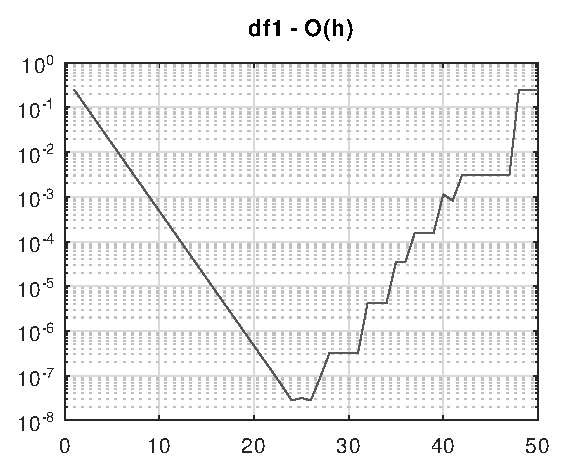
\includegraphics [width=0.65\textwidth]{../img/df1}\\ 
			\caption{График погрешностей  \label{fig.1}}
		\end{figure}
	
	
	\[r_{min} = 2.7963\cdot 10^{-8},~ \text{при} ~ k=24, h_k=1.1921\cdot 10^{-7}\]
	\newpage
	
	\section{Первая конечно разностная производная 2-го порядка точности}
		\begin{flushright}
			Таблица 2. Погрешности первой производной второго порядка точности.
		\end{flushright}
		
		
		\begin{table}[h!]
			\centering
			\begin{tabular}{|c|c|c|}
				\hline
				$k$  & $h_k$       & $r_k$        \\ \hline
				13 & 0.00024414 & 3.2859e-10  \\ \hline
				14 & 0.00012207 & 8.1203e-11  \\ \hline
				15 & 6.1035e-05 & 2.2996e-11  \\ \hline
				16 & 3.0518e-05 & -3.5212e-11 \\ \hline
				17 & 1.5259e-05 & 2.2996e-11  \\ \hline
				18 & 7.6294e-06 & 2.2996e-11  \\ \hline
				19 & 3.8147e-06 & 2.2996e-11  \\ \hline
				20 & 1.9073e-06 & 2.2996e-11  \\ \hline
				21 & 9.5367e-07 & 2.2996e-11  \\ \hline
				22 & 4.7684e-07 & 1.8856e-09  \\ \hline
				23 & 2.3842e-07 & -1.8396e-09 \\ \hline
				24 & 1.1921e-07 & -1.8396e-09 \\ \hline
				25 & 5.9605e-08 & -1.8396e-09 \\ \hline
				26 & 2.9802e-08 & 2.7963e-08  \\ \hline
				27 & 1.4901e-08 & 2.7963e-08  \\ \hline
				28 & 7.4506e-09 & -9.1247e-08 \\ \hline
				29 & 3.7253e-09 & 1.4717e-07  \\ \hline
				30 & 1.8626e-09 & -3.2967e-07 \\ \hline
				31 & 9.3132e-10 & -3.2967e-07 \\ \hline
				32 & 4.6566e-10 & -3.2967e-07 \\ \hline
				33 & 2.3283e-10 & -4.1444e-06 \\ \hline
				34 & 1.1642e-10 & -4.1444e-06 \\ \hline
			\end{tabular}
		\end{table}
		
		
		
	\newpage
	\begin{figure}[h!] 
		\centering
		\renewcommand{\figurename}{Рисунок}
		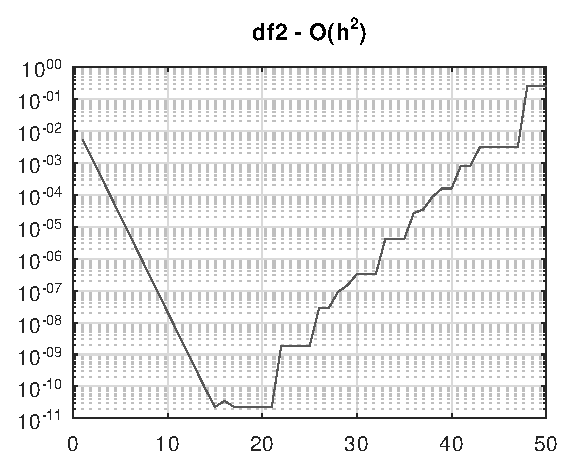
\includegraphics [width=0.65\textwidth]{../img/df2}\\ 
		\caption{График погрешностей  \label{fig.2}}
	\end{figure}
	
	
	\[r_{min} = -2.2996\cdot 10^{-11},~ \text{при} ~ k=15, h_k=6.1035\cdot 10^{-5}\]
	
	\section{Первая конечно разностна производная 4-го порядка точности}
	
		\begin{flushright}
			Таблица 3. Погрешности первой производной четвёртого порядка точности.
		\end{flushright}
		\begin{table}[h!]
			\centering
			\begin{tabular}{|c|c|c|}
				\hline
				$k$  & $h_k$       & $r_k$        \\ \hline
				1  & 1          & 0.00033548  \\ \hline
				2  & 0.5        & 2.2119e-05  \\ \hline
				3  & 0.25       & 1.4014e-06  \\ \hline
				4  & 0.125      & 8.7886e-08  \\ \hline
				5  & 0.0625     & 5.4976e-09  \\ \hline
				6  & 0.03125    & 3.4374e-10  \\ \hline
				7  & 0.015625   & 2.1347e-11  \\ \hline
				8  & 0.0078125  & 1.6225e-12  \\ \hline
				9  & 0.0039062  & -1.2071e-13 \\ \hline
			\end{tabular}
		\end{table}


		\begin{table}[h!]
			\centering
			\begin{tabular}{|c|c|c|}
				\hline
		
					10 & 0.0019531  & 8.6456e-13  \\ \hline
					11 & 0.00097656 & 2.5824e-13  \\ \hline
					12 & 0.00048828 & -1.2576e-12 \\ \hline
					13 & 0.00024414 & 8.4437e-12  \\ \hline
					14 & 0.00012207 & -8.5335e-12 \\ \hline
					15 & 6.1035e-05 & -1.2576e-12 \\ \hline
					16 & 3.0518e-05 & -4.4913e-11 \\ \hline
					17 & 1.5259e-05 & 6.1801e-11  \\ \hline
					18 & 7.6294e-06 & -1.3222e-10 \\ \hline
					19 & 3.8147e-06 & -1.3222e-10 \\ \hline
				\end{tabular}
		\end{table}


		\begin{figure}[h!] 
			\centering
			\renewcommand{\figurename}{Рисунок}
			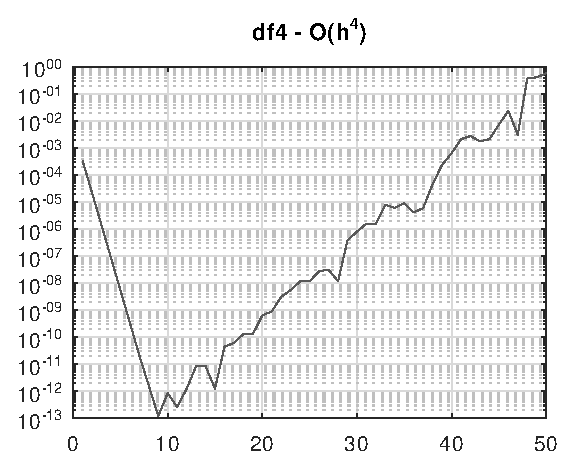
\includegraphics [width=0.65\textwidth]{../img/df4}\\ 
			\caption{График погрешностей  \label{fig.3}}
		\end{figure}
		
		
		\[r_{min} = -1.2071\cdot 10^{-13},~ \text{при} ~ k=9, h_k=0.0039062\]
		\newpage
	
	\section{Вторая конечно разностна производная 2-го порядка точности}
	
	\begin{flushright}
		Таблица 4. Погрешности второй производной второго порядка точности.
	\end{flushright}
	\begin{table}[h!]
		\centering
		\begin{tabular}{|c|c|c|}
			\hline
			$k$  & $h_k$       & $r_k$        \\ \hline
			1  & 1          & -0.0052484  \\ \hline
			2  & 0.5        & -0.0013226  \\ \hline
			3  & 0.25       & -0.00033132 \\ \hline
			4  & 0.125      & -8.2873e-05 \\ \hline
			5  & 0.0625     & -2.0721e-05 \\ \hline
			6  & 0.03125    & -5.1804e-06 \\ \hline
			7  & 0.015625   & -1.2951e-06 \\ \hline
			8  & 0.0078125  & -3.2379e-07 \\ \hline
			9  & 0.0039062  & -8.106e-08  \\ \hline
			10 & 0.0019531  & -2.0059e-08 \\ \hline
			11 & 0.00097656 & -7.9514e-09 \\ \hline
			12 & 0.00048828 & -7.9514e-09 \\ \hline
			13 & 0.00024414 & -5.2655e-08 \\ \hline
			14 & 0.00012207 & -2.9107e-07 \\ \hline
			15 & 6.1035e-05 & 1.8576e-07  \\ \hline
			16 & 3.0518e-05 & -1.7216e-06 \\ \hline
			17 & 1.5259e-05 & 2.0931e-06  \\ \hline
			18 & 7.6294e-06 & -5.8942e-05 \\ \hline
			19 & 3.8147e-06 & -5.8942e-05 \\ \hline
			20 & 1.9073e-06 & -5.8942e-05 \\ \hline
			21 & 9.5367e-07 & -5.8942e-05 \\ \hline
			
		\end{tabular}
	\end{table}
	\newpage
	\begin{figure}[h!] 
		\centering
		\renewcommand{\figurename}{Рисунок}
		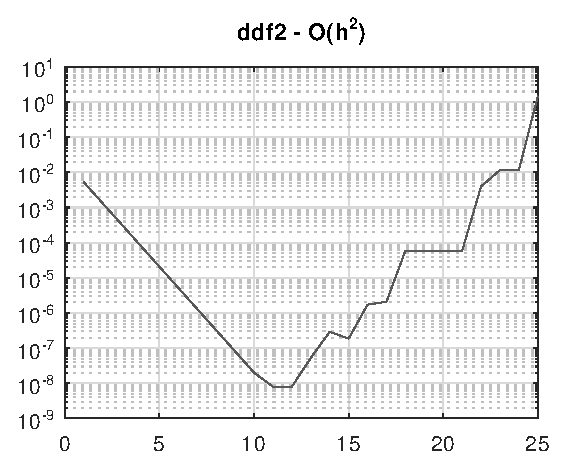
\includegraphics [width=0.65\textwidth]{../img/ddf1}\\ 
		\caption{График погрешностей  \label{fig.4}}
	\end{figure}

	
	\[r_{min} = -7.9514\cdot 10^{-9},~ \text{при} ~ k=11, h_k=0.00097656\]
	
	\section{Вторая конечно разностна производная 4-го порядка точности}
	
	\begin{flushright}
		Таблица 5. Погрешности второй производной четвертого порядка точности.
	\end{flushright}
	
	\begin{table}[h!]
		\centering
		\begin{tabular}{|c|c|c|}
			
			\hline
			$k$  & $h_k$       & $r_k$        \\ \hline
			1  & 1          & -0.0002162  \\ \hline
			2  & 0.5        & -1.4048e-05 \\ \hline
			3  & 0.25       & -8.8674e-07 \\ \hline
			4  & 0.125      & -5.5559e-08 \\ \hline
			5  & 0.0625     & -3.4751e-09 \\ \hline
			6  & 0.03125    & -2.1946e-10 \\ \hline
			7  & 0.015625   & -3.6345e-11 \\ \hline
			8  & 0.0078125  & -5.4535e-11 \\ \hline
			9  & 0.0039062  & -3.2617e-10 \\ \hline
			
		\end{tabular}
	\end{table}
	
	\begin{table}[h!]
		\centering
		\begin{tabular}{|c|c|c|}
			\hline
			10 & 0.0019531  & 2.7531e-10  \\ \hline
			11 & 0.00097656 & -7.0201e-09 \\ \hline
			12 & 0.00048828 & -2.2853e-08 \\ \hline
			13 & 0.00024414 & -1.1226e-07 \\ \hline
			14 & 0.00012207 & -3.5068e-07 \\ \hline
			15 & 6.1035e-05 & -5.2655e-08 \\ \hline
			16 & 3.0518e-05 & -3.311e-06  \\ \hline
			17 & 1.5259e-05 & -1.0623e-05 \\ \hline
			18 & 7.6294e-06 & -0.00011998 \\ \hline
		\end{tabular}
	\end{table}

	\begin{figure}[h!] 
		\centering
		\renewcommand{\figurename}{Рисунок}
		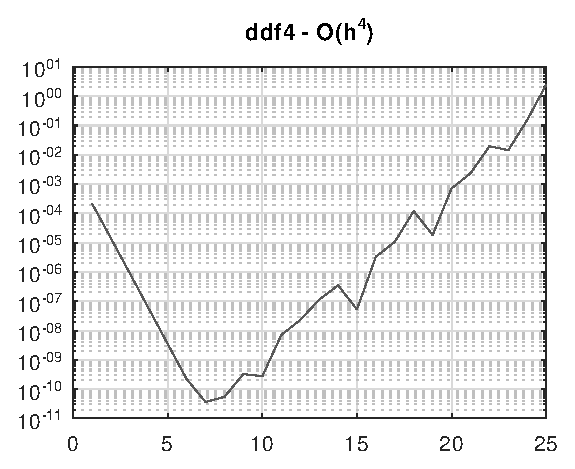
\includegraphics [width=0.65\textwidth]{../img/ddf4}\\ 
		\caption{График погрешностей  \label{fig.5}}
	\end{figure}
	
	
	\[r_{min} = -3.6345\cdot 10^{-11},~ \text{при} ~ k=7, h_k=0.015625\]

\lstset{language=Matlab,%
	%basicstyle=\color{red},
	breaklines=true,%
	morekeywords={matlab2tikz},
	keywordstyle=\color{blue},%
	morekeywords=[2]{1}, keywordstyle=[2]{\color{black}},
	identifierstyle=\color{black},%
	stringstyle=\color{mylilas},
	commentstyle=\color{mygreen},%
	showstringspaces=false,%without this there will be a symbol in the places where there is a space
	numbers=left,%
	numberstyle={\small \color{black}},% size of the numbers
	numbersep=9pt, % this defines how far the numbers are from the text
	emph=[1]{for,end,break},emphstyle=[1]\color{red}, %some words to emphasise
	%emph=[2]{word1,word2}, emphstyle=[2]{style},    
}

	\newpage
	\section{Листинг функций и сценариев}
	\subsection{f.m}
	\lstinputlisting{../f.m}
	\subsection{df.m}
	\lstinputlisting{../df.m}
	\subsection{df1.m}
	\lstinputlisting{../df1.m}
	\subsection{df2.m}
	\lstinputlisting{../df2.m}
	\subsection{df4.m}
	\lstinputlisting{../df4.m}
	\subsection{ddf.m}
	\lstinputlisting{../ddf.m}
	\subsection{ddf1.m}
	\lstinputlisting{../ddf1.m}
	\subsection{ddf4.m}
	\lstinputlisting{../ddf4.m}
	
	\subsection{ww1.m}
	\lstinputlisting{../ww1.m}
	\subsection{ww2.m}
	\lstinputlisting{../ww2.m}
	\subsection{ww4.m}
	\lstinputlisting{../ww4.m}
	\subsection{ww21.m}
	\lstinputlisting{../ww21.m}
	\subsection{ww24.m}
	\lstinputlisting{../ww24.m}


	\end{document}